\section{Problem description}
\begin{figure}
\centering
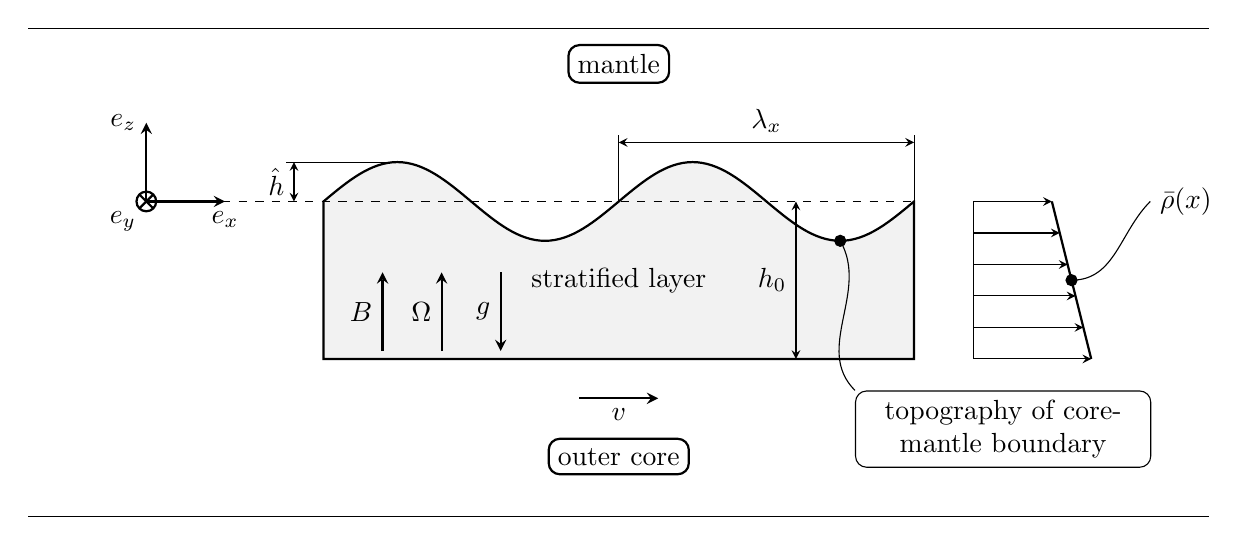
\begin{tikzpicture}[>=stealth]
	\pgfmathsetmacro\a{0.5}
	\pgfmathsetmacro\e{1.0}
	\pgfmathsetmacro\d{0.1}
	\pgfmathsetmacro\r{0.125}
	\pgfmathsetmacro\h{2.}
	\pgfmathsetmacro\b{7.5}
	\begin{scope}[shift={(-0.8*\b,\h)}]
		\draw[thick,<->] (0,\e) node[left]{$\bm{e}_z$} |- (\e,0) node[below]{$\bm{e}_x$};
		\draw[thick] (0,0) circle[radius=\r] node[below left]{$\bm{e}_y$};
		\draw[thick] (225:\r) -- (45:\r);
		\draw[thick] (135:\r) -- (-45:\r);
	\end{scope}
	% geometry
	\draw[shift={(-0.5*\b,\h)},thick,xscale=0.125*\b,fill=gray!10] (0,0) 
		sin (1,\a) cos (2,0) sin (3,-\a) cos (4,0) 
		sin (5,\a) cos (6,0) sin (7,-\a) cos (8,0) 
		-| (8,-\h) |-(0,-\h) -| cycle;
	\draw[dashed] (-0.7*\b,\h) -- (0.5*\b,\h);
	\draw[fill] (.375*\b,\h-\a) circle[radius=2pt];
	% dimensions
	\draw[<->] (0.3*\b,0) --node[midway,left]{$h_0$} (0.3*\b,\h);
	\draw (-0.375*\b,\h+\a) -- (-0.55*\b-\d,\h+\a);
	\draw[<->] (-0.55*\b,\h) --node[midway,left]{$\hat{h}$} (-0.55*\b,\h+\a);
	\draw[<->] (0,\h+1.5*\a) --node[midway,above]{$\lambda_x$} (0.5*\b,\h+1.5*\a);
	\draw (0.5*\b,\h) -- (0.5*\b,\h+1.5*\a+\d);
	\draw (0,\h) -- (0,\h+1.5*\a+\d);
	\draw (0.6*\b,0) -- (0.6*\b,\h);
	\draw[thick] (0.6*\b+1.5*\e,0) -- (0.6*\b+\e,\h);
	\foreach \i in {0,...,5}
	{
		\draw[->] (0.6*\b,\i*0.2*\h) -- (0.6*\b+1.5*\e-\i*0.1*\e,\i*0.2*\h);
	}
	% annotations
	\draw (-\b,2.1*\h) -- (\b,2.1*\h);
	\draw (-\b,-\h) -- (\b,-\h);
	\node[draw,below,thick,rounded corners] at (0,-0.5*\h) {outer core};
	\node[draw,below,thick,rounded corners] at (0,\h+4*\a) {mantle};
	\node at (0,0.5*\h) {stratified layer};
	\draw (.375*\b,\h-\a) to[in=135,out=-60] (0.4*\b,-0.2*\h) node[draw,rounded corners,text width=10em,anchor=north west,text centered]{topography of core-mantle boundary};
	\draw[fill] (0.6*\b+\e+0.25*\e,0.5*\h) circle[radius=2pt];
	\draw (0.6*\b+\e+0.25*\e,0.5*\h) to[out=0,in=225] (0.7*\b+1.5*\e,\h) node[right]{$\bar{\rho}(\bm{x})$};
	\draw[->,thick] (-0.3*\b,\d) --node[midway,left]{$\bm{\Omega}$} (-0.3*\b,\e+\d);
	\draw[->,thick] (-0.4*\b,\d) --node[midway,left]{$\bm{B}$} (-0.4*\b,\e+\d);
	\draw[<-,thick] (-0.2*\b,\d) --node[midway,left]{$\bm{g}$} (-0.2*\b,\e+\d);
	\draw[->,thick] (-0.5*\e,-\a) --node[midway,below]{$\bm{v}$} (0.5*\e,-\a);
\end{tikzpicture}
\caption{Sketch of the stratified fluid layer at the core-mantle boundary. }
\end{figure}

The basic equations describing the problem are given by the \textsc{Navier}-\textsc{Stokes} equations using the \textsc{Boussinesq} approximation accompanied by the magnetic induction equation. The system is considered in rotating reference frame and the constant angular velocity is given by $\bm{\Omega}=\Omega\ez$ and its magnitude is the angular velocity of the Earth. Furthermore, the gravitational acceleration is given by $\bm{g}=-g\ez$. This system reads:
\begin{gather}
	\nabla\cdot\bm{v}=0\,, \qquad
	\rho_0\Big(\bm{v}\cdot(\nabla\otimes\bm{v})+2\bm{\Omega}\times\bm{v}\Big)=-\nabla P+\rho\bm{g}+\frac{1}{\gmu_0}\bm{B}\cdot\nabla\otimes\bm{B}\,,\\
	\nabla\cdot\bm{B}=0\,, \qquad
	\nabla\times\left(\bm{v}\times\bm{B}\right)+\eta\laplace\bm{B}=\bm{0}\,.
\end{gather}
The perturbation of the system is given by
\begin{equation}
	\rho=\bar{\rho}+\rho'\,,\qquad
	\bm{v}=\bar{\bm{V}}+\bm{v}'\,,\qquad 
	P=\bar{P}+p'\,,\qquad
	\bm{B}=\bar{\bm{B}}+\bm{b}'\,,
\end{equation}
Substitution and neglecting the non-linear terms gives the system
\begin{subequations}
\begin{gather}
	\nabla\cdot\bm{v}'=0\,,\qquad \nabla\cdot\bm{b}'=0\,,\\
	\begin{multlined}
	\rho_0\Big(\bar{\bm{V}}\cdot(\nabla\otimes\bm{v}')+\bm{v}'\cdot(\nabla\otimes\bar{\bm{V}})+\bm{v}'\cdot(\nabla\otimes\bm{v}')+2\bm{\Omega}\times\bm{v}'\Big)\\
	\hspace{3cm}=-\nabla p'+\rho'\bm{g}+\frac{1}{\gmu_0}\left(\bar{\bm{B}}\cdot(\nabla\otimes\bm{b}')+\bm{b}'\cdot(\nabla\otimes\bar{\bm{B}})+\bm{b}'\cdot(\nabla\otimes\bm{b}')\right)\,,
	\end{multlined}\\
	\nabla\times\big(\bm{v}'\times\bar{\bm{B}}\big)+\nabla\times\left(\bar{\bm{V}}\times\bm{b}'\right)+\nabla\times\left(\bm{v}'\times\bm{b}'\right)+\eta\laplace\bm{b}'=\bm{0}\,,\\
	\bar{\bm{V}}\cdot\nabla\rho'+\bm{v}'\cdot\nabla\bar{\rho}+\bm{v}'\cdot\nabla\rho'=0\,.
\end{gather}
\end{subequations}
The reference scales are chosen as $\lref=\lambda_x$, $\rhoref=\rho_0$, $\vref=\norm{\bar{\bm{V}}}$, $\Bref=\norm{\bar{\bm{B}}}$, $\gref=\norm{\bm{g}}$. With
\begin{equation}
	\hat{\bm{x}}=\frac{\bm{x}}{\lref}\,,\quad
	\hat{\rho}=\frac{\rho'}{\rhoref}\,,\quad
	\hat{\bm{v}}=\frac{\bm{v}'}{\vref}\,,\quad 
	\hat{p}=\frac{p'}{\rhoref\vref^2}\,,\quad
	\hat{\bm{b}}=\frac{\bm{b}'}{\Bref}\,,\quad
	\hat{\bm{g}}=\frac{\bm{g}}{\gref}\,,
\end{equation}
the dimensionless form is given by
\begin{subequations}
\begin{gather}
	\hat{\nabla}\cdot\hat{\bm{v}}=0\,,\qquad \hat{\nabla}\cdot\hat{\bm{b}}=0\,,\\
	\begin{multlined}
	\hat{\bm{V}}\cdot(\hat{\nabla}\otimes\hat{\bm{v}})+\hat{\bm{v}}\cdot(\hat{\nabla}\otimes\hat{\bm{V}})+\hat {\bm{v}}\cdot(\hat{\nabla}\otimes\hat{\bm{v}})+\frac{1}{\Rossby} 2\hat{\bm{\Omega}}\times\hat{\bm{v}}\\
	\hspace{2.75cm}=-\hat{\nabla} \hat{p}+\frac{1}{\Froude^2}\hat{\rho}\hat{\bm{g}}+\Alfven^2\left(\hat{\bm{B}}\cdot(\hat{\nabla}\otimes\hat{\bm{b}})+\hat{\bm{b}}\cdot(\hat{\nabla}\otimes\hat{\bm{B}})+\hat{\bm{b}}\cdot(\hat{\nabla}\otimes\hat{\bm{b}})\right)\,,
	\end{multlined}\\
	\MagneticReynolds\left[\hat{\nabla}\times(\hat{\bm{v}}\times\hat{\bm{B}})+\hat{\nabla}\times(\hat{\bm{V}}\times\hat{\bm{b}})+\hat{\nabla}\times(\hat{\bm{v}}\times\hat{\bm{b}})\right]+\hat{\laplace}\hat{\bm{b}}=\bm{0}\,,\\
	\hat{\bm{V}}\cdot\hat{\nabla}\hat{\rho}-\frac{N^2\lref}{\gref}\hat{\bm{v}}\cdot\bm{e}_z+\hat{\bm{v}}\cdot\hat{\nabla}\hat{\rho}=0\,.
\end{gather}
\end{subequations}
The dimensionless number are given by
\begin{equation}
	\Rossby=\frac{\vref}{\Omega\lref}\,,\quad
	\Froude=\frac{\vref}{\sqrt{\gref\lref}}\,,\quad
	\Alfven=\frac{V_\mathrm{A}}{\vref}\,,\quad 
	\MagneticReynolds=\frac{\vref\lref}{\eta}\,,
\end{equation}
where $V_\mathrm{A}=\Bref/\sqrt{\rhoref\mu}$ is the Alfv\'en velocity.

From now on, we omit the circumflex to indicate a dimensionless quantity.

We introduce the following short-hand notations for volume and surface integrals
\begin{equation*}
	\inner{\bm A}{\bm B} = \int\limits_{\Omega} \bm A \star \bm B\, \d V \; , \quad
	\innerSurf{\bm A}{\bm B}  = \int\limits_{\Gamma} \bm A \star \bm B\, \d A \ ,
\end{equation*}
where $\bm A \star \bm B$ represents the contraction of two tensors $\bm A$ and $\bm B$ of arbitrary rank to a scalar. Furthermore, we introduce operators related to viscosity/diffusion~($\mathcal{A}$), incompressible/pressure~($\mathcal{B}$) and convection~($\mathcal{C}$).
\begin{align*}
\begin{aligned}
	\elliptic{\bm{\phi}}{\bm{\psi}}&=\inner{\nabla\bm{\phi}}{\nabla\bm{\psi}}\,, &
	\saddle{\bm{\phi}}{\psi}&=\inner{\nabla\cdot\bm{\phi}}{\psi}\,, &
	\convec{\bm{\phi}}{\bm{\psi}}{\bm{\chi}}&=\inner{\bm{\phi} \cdot (\nabla\bm{\psi})}{\bm{\chi}}\,.
\end{aligned}
\end{align*}

\section{Weak form of the continuity equation}
Because $\nabla\cdot\bm{V}=0$ and  $\nabla\cdot\bm{v}'=0$, the continuity can be written in conservative form:
\begin{equation}
	\nabla\cdot(\rho'(\bm{V}+\bm{v}'))=\frac{N^2\lref}{\gref}\bm{v}'\cdot\ez\,.
\end{equation}
Multiplication with a test function~$r$ and integration by parts gives:
\begin{equation}
	-\inner{\rho'(\bm{V}+\bm{v}')}{\nabla r}+\innerSurf{\bm{n}\cdot\rho(\bm{V}+\bm{v})}{r}=\frac{N^2\lref}{\gref}\inner{\bm{v}\cdot\ez}{r}\,.
\end{equation}
The weak form augmented with the entropy viscosity~$\nu_\mathrm{E}$ is given by
\begin{equation}
	\inner{\nu_\mathrm{E}\nabla\rho'}{\nabla r}-\inner{\rho'(\bm{V}+\bm{v}')}{\nabla r}+\innerSurf{\bm{n}\cdot\rho(\bm{V}+\bm{v})}{r}=\frac{N^2\lref}{\gref}\inner{\bm{v}\cdot\ez}{r}\,.
\end{equation}

\section{Weak form of the momentum equation}
If the compressibility and momentum equations are multiplied by testfunctions~$q$ and $\bm{w}$. After integrating the pressure by parts, the weak form reads:
\begin{gather}
	\saddle{\bm{v}'}{q}=0\,,\label{eqn:WeakIncompressibility} \\
	\begin{multlined}
	\convec{\bm{V}}{\bm{v}'}{\bm{w}}+\convec{\bm{v}'}{\bm{V}}{\bm{w}}+\convec{\bm{v}'}{\bm{v}'}{\bm{w}}+\frac{1}{\Rossby}\inner{2\bm{\Omega}\times\bm{v}'}{\bm{w}}\\
	=\saddle{\bm{w}}{p'}-\innerSurf{p'\bm{n}}{\bm{w}}+\frac{1}{\Froude^2}\inner{\rho'\bm{g}}{\bm{w}}+{}\\
	{}+\Alfven\left(\convec{\bm{B}}{\bm{b}'}{\bm{w}}+\convec{\bm{b}'}{\bm{B}}{\bm{w}}+\convec{\bm{b}'}{\bm{b}'}{\bm{w}}\right)\,,
	\end{multlined}\label{eqn:WeakMomentum}
\end{gather}

As outlined below, we will introduce a vector potential for the magnetic field, \ie $\bm{b}'=\nabla\times\bm{A}$. This causes problems in the Lorentz force term because a second derivative appears:
\begin{equation}
	\bm{b}'\cdot(\nabla\otimes\bm{b}')\cdot\bm{w}=(\nabla\times\bm{A})\cdot[\nabla\otimes(\nabla\times\bm{A})]\cdot\bm{w}\,.
\end{equation}
This derivative is not properly defined and therefore this term must also be integrated by parts. Note that
\begin{equation}
	\nabla\cdot((\bm{b}\cdot\bm{c})\bm{a})=(\nabla\cdot\bm{a})(\bm{b}\cdot\bm{c})+\bm{a}\cdot(\nabla\otimes\bm{b})\cdot\bm{c}+\bm{a}\cdot(\nabla\otimes\bm{c})\cdot\bm{b}\,.
\end{equation}
By substituting $\bm{a},\bm{b}\rightarrow\bm{b}'$ and $\bm{c}\rightarrow\bm{w}$ and applying $\nabla\cdot\bm{b}'=0$, we obtain the following expression for the Lorentz force:
\begin{equation}
	\bm{b}'\cdot(\nabla\otimes\bm{b}')\cdot\bm{w}=\nabla\cdot((\bm{b}\cdot\bm{c})\bm{a})-\bm{b}'\cdot(\nabla\otimes\bm{w})\cdot\bm{b}'\,,
\end{equation}
which eliminates the derivative on the magnetic field. Substituting the magnetic vector potential and applying the divergence theorem gives:
\begin{equation}
	\convec{\bm{b}'}{\bm{b}'}{\bm{w}}=\innerSurf{\bm{n}\cdot(\nabla\times\bm{A})}{(\nabla\times\bm{A})\cdot\bm{w}}-\convec{\nabla\times\bm{A}}{\bm{w}}{\nabla\times\bm{A}}
\end{equation}
Hence, the weak of the momentum equation reads
\begin{multline}
	\convec{\bm{V}}{\bm{v}'}{\bm{w}}+\convec{\bm{v}'}{\bm{V}}{\bm{w}}+\convec{\bm{v}'}{\bm{v}'}{\bm{w}}+\frac{1}{\Rossby}\inner{2\bm{\Omega}\times\bm{v}'}{\bm{w}}\\
	=\saddle{\bm{w}}{p'}-\innerSurf{p'\bm{n}}{\bm{w}}+\frac{1}{\Froude^2}\inner{\rho'\bm{g}}{\bm{w}}-\Alfven\left(\convec{\bm{B}}{\bm{w}}{\bm{b}'}+\convec{\bm{b}'}{\bm{w}}{\bm{B}}+\convec{\bm{b}'}{\bm{w}}{\bm{b}'}\right)+{}\\
	{}+\Alfven\left(\innerSurf{\bm{n}\cdot\bm{B}}{\bm{b}'\cdot\bm{w}}+\innerSurf{\bm{n}\cdot\bm{b}'}{\bm{B}\cdot\bm{w}}+\innerSurf{\bm{n}\cdot\bm{b}'}{\bm{b}'\cdot\bm{w}}\right)\,,
\end{multline}

\section{Weak form of the induction equation}
The magnetic field is expressed through a vector potential~$\bm{A}$. We derive the weak from the stationary Maxwell equations:
\begin{equation}
	\nabla\cdot\bm{B}=0\,,\qquad
	\nabla\times\bm{E}=0\,,\qquad
	-\nabla\times\bm{H}=\sigma(\bm{E}+\bm{v}\times\bm{B})
\end{equation}
The electric field and the magnetic are through: $\bm{E}=-\nabla\varphi$ and $\bm{B}=\nabla\times\bm{A}$. Hence, Amp\`ere's law reads:
\begin{equation}
	\frac{1}{\mu\sigma}\nabla\times(\nabla\times\bm{A})=-\nabla\varphi+\bm{v}\times(\nabla\times\bm{A})
\end{equation}
Substituting the perturbations for the potentials
\begin{equation}
	\varphi=\bar{\varphi}+\varphi'\,,\qquad
	\bm{A}=\bar{\bm{A}}+\bm{a}'\,,
\end{equation}
gives the following dimensional equation:
\begin{equation}
	\frac{1}{\mu\sigma}\nabla\times(\nabla\times\bm{a}')=-\nabla\varphi'+\bar{\bm{V}}\times(\nabla\times\bm{a}')+\bm{v}'\times(\nabla\times\bar{\bm{A}})+\bm{v}'\times(\nabla\times\bm{a}')\,.
\end{equation}
In order to obtain a dimensionless form, the potentials are normalized by $\hat{\bm{A}}=\bm{A}/(\lref\Bref)$ and $\hat{\varphi}=\varphi/(\eta\Bref)$. Then the dimensionless equation reads:
\begin{equation}
	\nabla\times\nabla\times\bm{a}'=-\nabla\varphi'+\MagneticReynolds\left(\bar{\bm{V}}\times(\nabla\times\bm{a}')+\bm{v}'\times(\nabla\times\bar{\bm{A}})+\bm{v}'\times(\nabla\times\bm{a}')\right)\,.
\end{equation}
In order to obtain the weak form, we multiply this equation by the testfunction~$\bm{c}$. Integration by parts gives:
\begin{multline}
	-\inner{\nabla\times\bm{a}}{\nabla\times\bm{c}}-\innerSurf{\bm{n}\times(\nabla\times\bm{a})}{\bm{c}}+\saddle{\bm{c}}{\varphi}-\innerSurf{\varphi\bm{n}}{\bm{c}}+{}\\
	{}+\MagneticReynolds\left(\inner{\bm{V}\times(\nabla\times\bm{a})}{\bm{c}}+\inner{\bm{v}\times(\nabla\times\bm{A})}{\bm{c}}+\inner{\bm{v}\times(\nabla\times\bm{a})}{\bm{c}}\right)=0\,.
\end{multline}